\chapter{Spiking Models: Neurons \& Synapses}\label{ch_spiking}
\chapterauthor{Zo\"e Tosi,  Jeff Yoshimi}

% Discuss raster plots in Simbrain
% Add glossary items
% Some kind of overview paragraph for the chapter
% When Simbrain 4 comes out, integrate with the new material and documentation there
% Either broaden out to a computational neuroscience chapter, or add an additional comp neuro chapter

Neurons of higher animals (from \emph{drosophila} to \emph{homo sapiens}) are characterized by an all-or-nothing on/off response that propagates signals via discrete packets known as \textbf{action potentials (APs)}. APs are characterized by a sudden increase in the \textbf{membrane potential} of a cell, brought about by a positive feedback process. After a short period of time (typically $<$ 1 ms) other mechanisms in the cell rein in this positive feedback, causing a rapid decrease in membrane potential. When voltage across the cell membrane is plotted over time we see a sudden sharp increase, then a rapid decrease in electrical potential taking the form of a \textbf{spike} (see \ref{TSComp}). Canonically this spike in the membrane voltage travels down the axon of a neuron to its synaptic terminals where voltage sensitive processes cause neurotransmitters to be released into the synaptic cleft, where they are taken up by other cells. 
% Footnote on non-canonical case?

% Move winnowed thing to footnote and expand
Coming from an engineering or connectionist background this process may seem unfamiliar since ``neurons'' (perhaps better called ``nodes'') associated with canonical artificial neural networks take on continuous values. Explicitly stated or not these continuous values are typically understood to vaguely represent the firing rate (number of spikes produced in some time window) of neurons--if such things are even within the realm of consideration. It is the case that in simple organisms neurons do take on what are known as  ``graded potentials'', which can be accurately described by a continuous variable. However these organisms tend to be extremely small and simple such as \emph{C. Elegans}, a 1 mm flatworm for which all of the exactly 302 of its neurons and their connections are known. In higher animals the vast majority of neurons communicate via spikes and therefore any continuous variable assigned to represent the instantaneous activity of a neuron is in one way or another derived (using windowed or exponential averages, for example) or an indirect measure (e.g. a strong correlations between variables like excitatory conductance and firing rate) \cite{o2016leabra}. Collectively the set of techniques for converting the activity of a spiking neuron into a single continuous value representing that activity is known as \textbf{rate-coding}. As it stands there is no clear consensus as to the importance of precise spike timings versus generalized rate-coded activity when studying information processing in the brain.
% Did not seem needed. However there is clearly a need to simulate spikes and other neural dynamics in order to fully account for neural behavior (regardless of whether or not the emphasis is on spike or rate-coded activations). 

What do we want out of a neuron model? The answer to this depends upon the question(s) we are interested in. Given that this chapter focuses on ``spiking neurons'' we will assume that at the very minimum the questions of interest require that APs not be abstracted away regardless of our use of rate-coding. From there we have a great many choices, which will be covered in detail later in the chapter. If this minimum criteria of ``produces spikes'' is our only criteria then highly simplified models scarcely different from the nodes of an ANN will fit the bill. Alternatively we may be interested in the particulars of some aspect of neural dynamics or require that our neurons' voltage waveforms during spikes correspond to those found in nature. If that is the case then our neuron model must itself be a complex entity with multiple variables governed by a set of coupled differential equations. Regardless of the complexity our biological models must replicate the basic functions of a neuron, which entails more than the neuron model itself. Contrary to what may be believed neurons and their functions can be understood in relatively simple terms. As a fundamental unit of the nervous system neurons 1) integrate inputs from neurons and/or some sensory stimulus 2) respond in some manner to that integrated input, and 3) propagate that output to other neurons or motor outputs. The models discussed thusfar represent (2) in this formulation. In this chapter we will be discussing both spiking/biological neuron models and how those neurons interact with other neurons via synapses ((1) and (3)).

\begin{figure}[h]
\centering
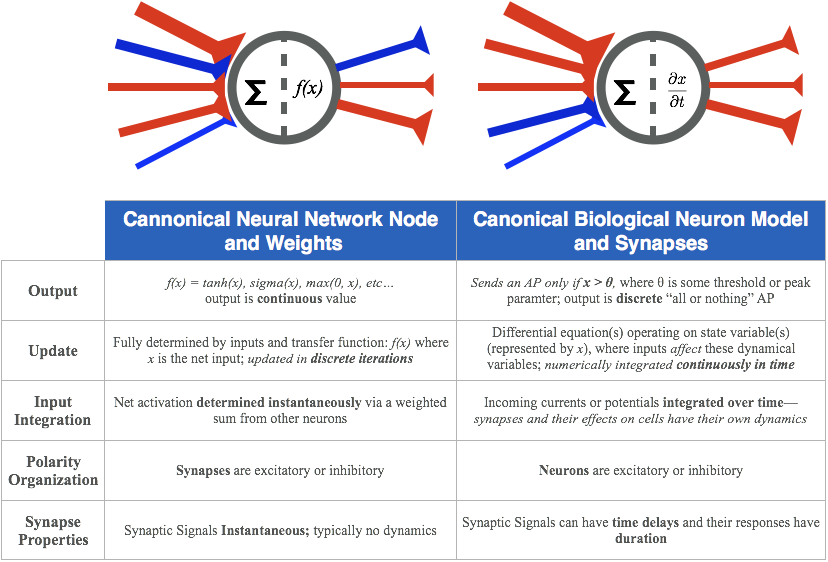
\includegraphics[width=\textwidth]{./images/NeuronComparison.png}
\caption[Simbrain Screenshot by Zo\"e Tosi ]{A broad comparison of neurons typically found in artificial neural networks and those found in computational neuroscience network models. These characterizations are not completely definitive, but can be thought of as describing the prototypical or canonical instantiation of each type.}
\label{NeuComp}
\end{figure}

\begin{figure}[h]
\centering
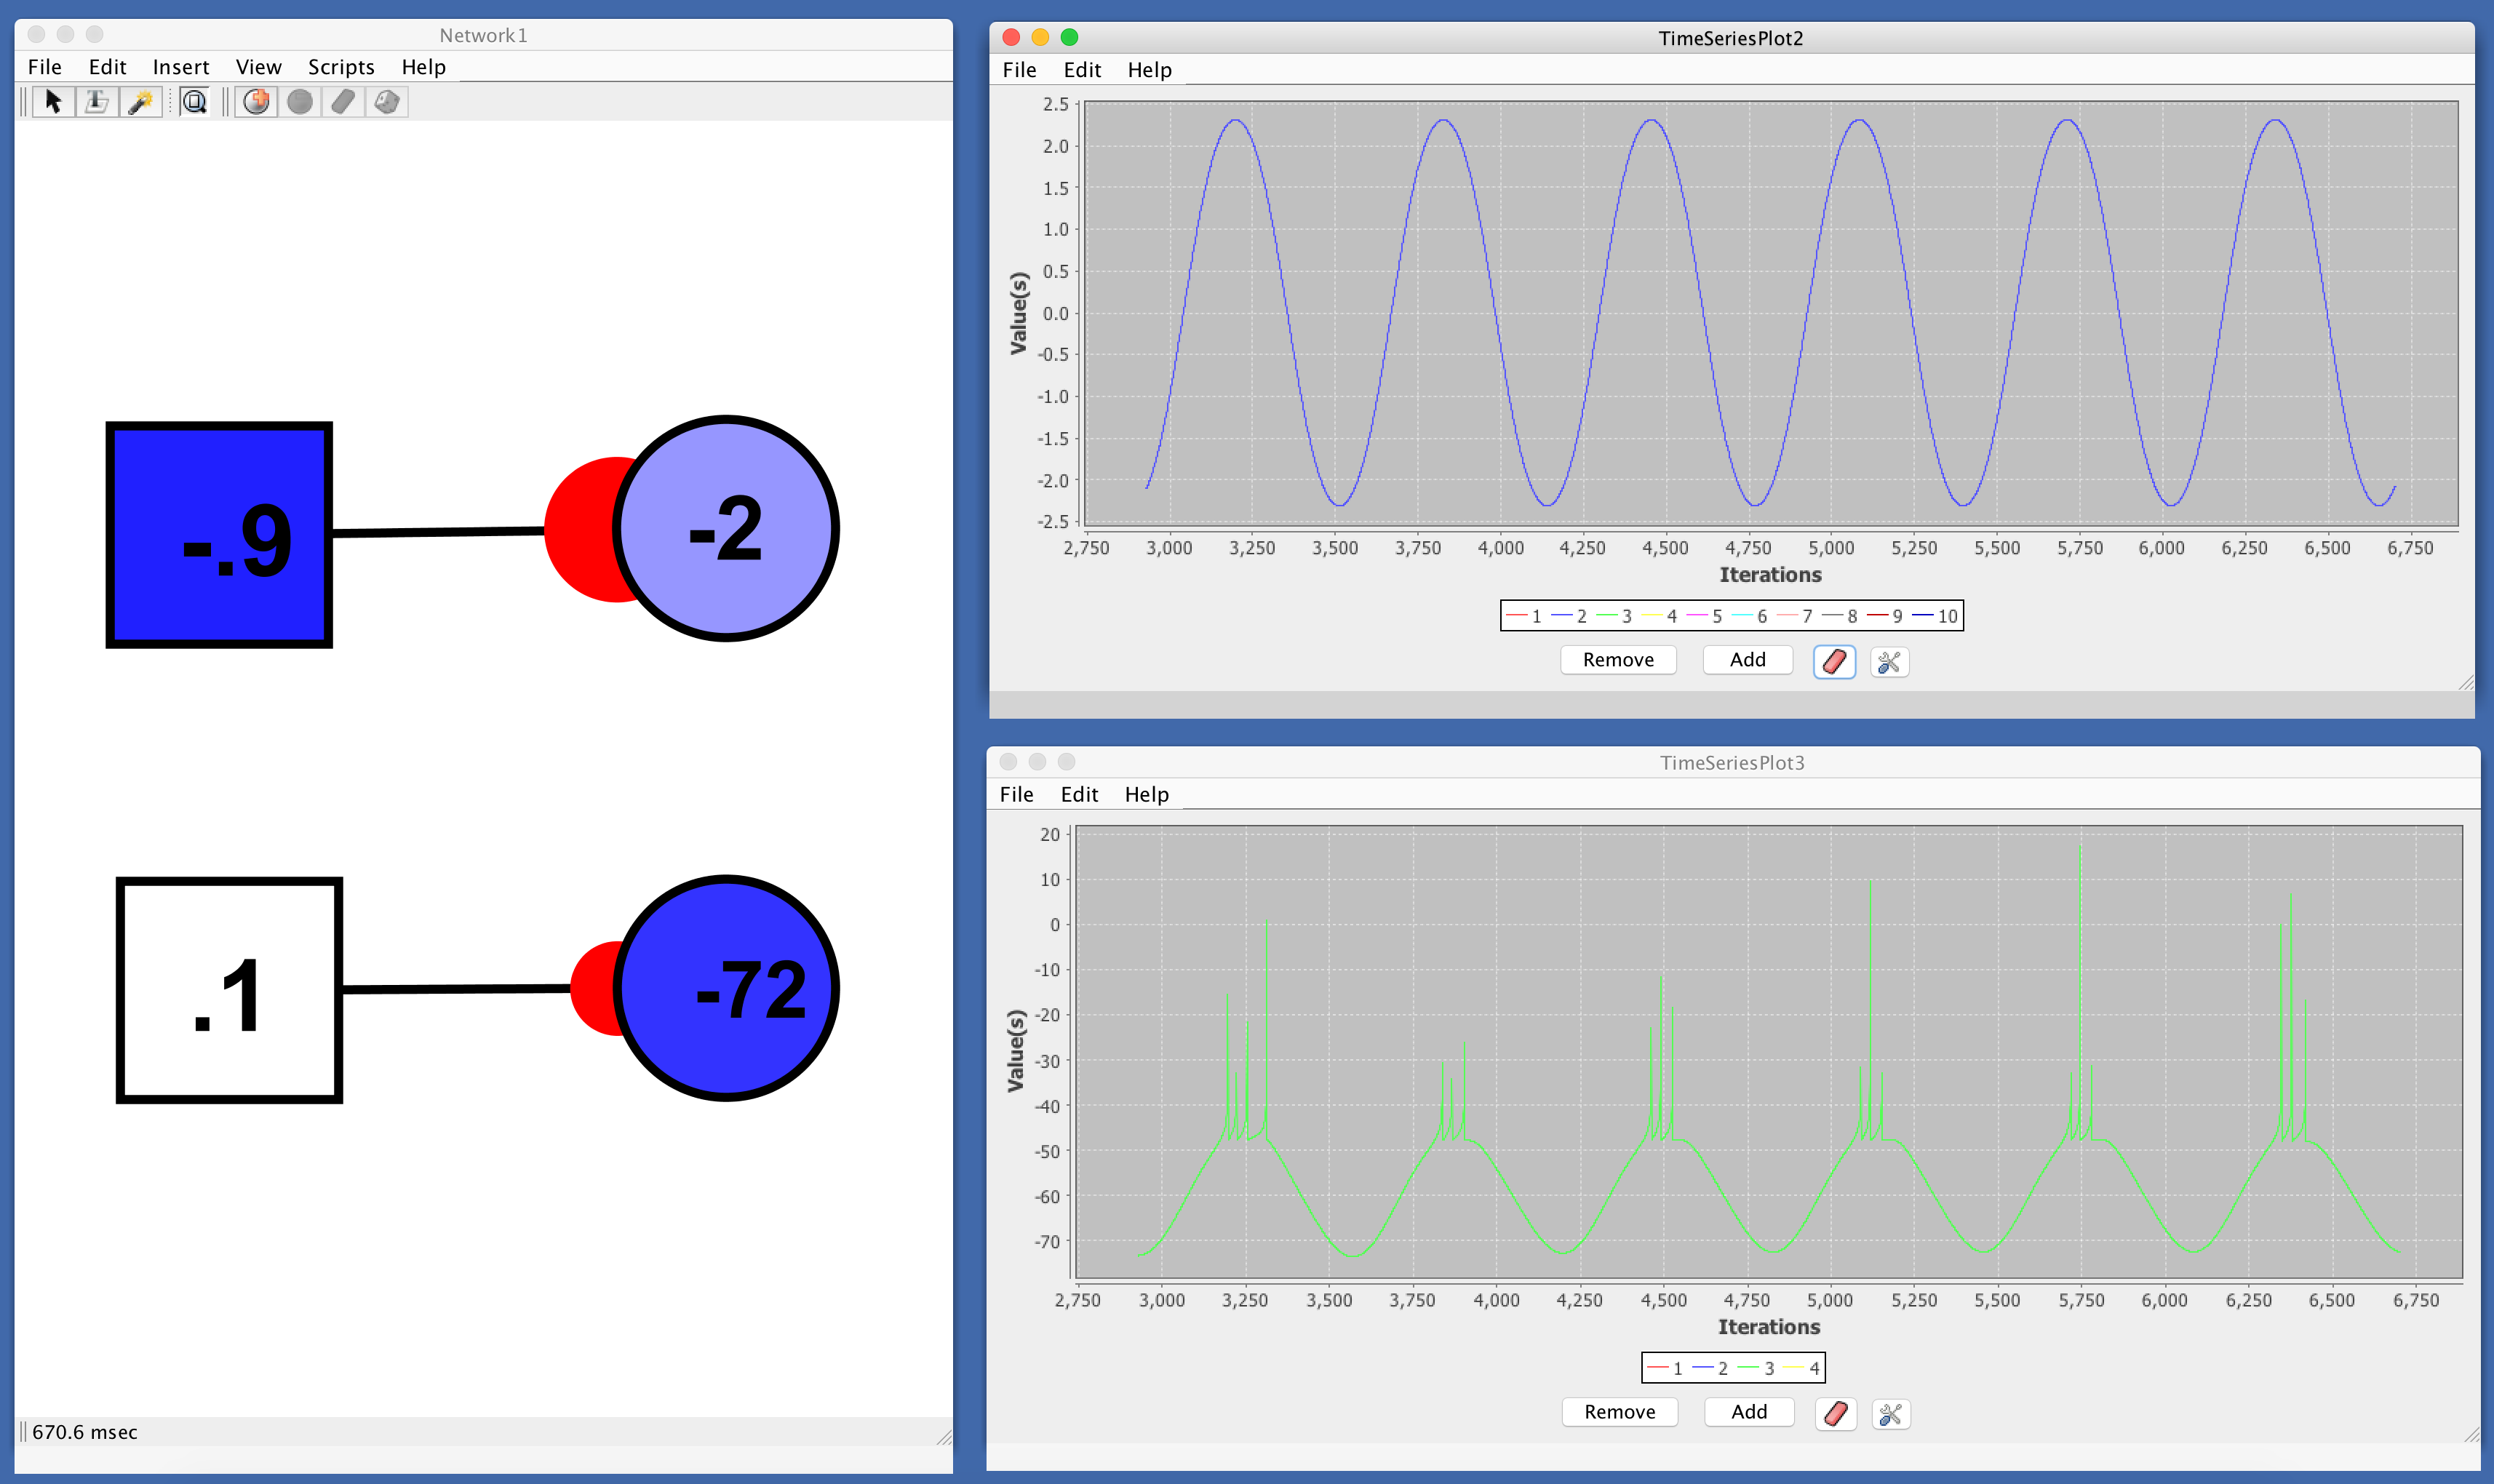
\includegraphics[width=\textwidth]{./images/SpikeNonSpikeTimeSeries.png}
\caption[Simbrain screenshot by Zo\"e Tosi]{A Simbrain desktop with two cells receiving inputs from activity generators. Both are providing the same sinusoidal input. Above is a typical connectionist neuron using a logistic activation function (bounded on (-5, 5)) , and below is a spiking neuron model. Across from each is a time series of activation (blue)  and membrane potential (mV; green) for the logistic and spiking neurons respectively. Notice the sharp increases and rapid decrease in membrane potential; these are ``spikes'' and if this neuron were connected to other neurons a signal would be propagating down the outgoing synapses. Also notice that the spikes are not the same in quantity or overall size and that there are small variations in their distance from one another. These are the result of the spiking neuron having its own internal dynamics unlike the logistic neuron.} 
\label{TSComp}
\end{figure}

\section{Level of abstraction}

Neurons are intrinsically complex entities when high levels of detail are taken into account, and indeed many computational neuroscientists have made neuron models that capture most or all of the relevant features of the cell. This involves modeling membrane potentials and ion channel dynamics for many different parts of a neuron. Models that do this are known as \emph{multi-compartment models}. This is further complicated by the large variety of neurons and their morphological and electrochemical differences. Depending on the questions one is interested in modeling with this level of detail may be required. 

Here are focusing on networks, so we focus on model neurons with no specific morphology. Thus we focus on \textbf{point neurons} (sometimes ``single-compartment'' neurons). Similarly a neuron may connect to another neuron via many different synaptic terminals that have different impacts on the target cell based on their strengths and locations (cell dendrites, soma, and the axon hillock being common). We only consider the impact of a single synaptic connection between two neurons, which stands in for this more complex relationship. In the literature the total change in a post-synaptic's membrane potential from a single axonal fiber is referred to as a unitary post-synaptic potential. 
	
Neurons are also associated with neurotransmitters, which have distinct functions. Synaptic receptors on the cell respond to specific neurotransmitters from other cells and can be divided into two classes: \textbf{Ionotropic} and \textbf{Metabotropic}. Ionotropic receptors are the simplest and are essentially ion channels on the surface of a cell that respond to a neurotransmitter by either opening or closing, thus rapidly having a direct, clear-cut impact on the membrane potential of the cell (see \extref{neuronsSynapses}). Most glutamate receptors (NMDA, AMPA, and kainate) and GABA$_A$ receptors are of this type and are excitatory and inhibitory, respectively. Metabotropic receptors on the other hand respond to neurotransmitters in complex long-term ways. When these receptors are activated a signal transduction pathway is set in motion that produces complex cellular and metabolic responses. Well-known neurotransmitters  such as Dopamine, Serotonin, Acetylcholine, and Norepinephrine typically use receptors of this type (see \extref{neuroModulator}). We focus on ionotropic neurotransmitters in this chapter.\footnote{Why abstract away so many potentially important features? The simple answer is that for many questions in neuroscience these details simply aren't necessary. This is particularly true of ``higher level'' phenomena. For instance a neuron's ability to store information about its past inputs can be explained without any reference to morphology, metabotropic neurotransmitter receptors, etc. \cite{maass2002computing}. Complex features of synaptic structure and firing patterns have also been explained via phenomenological models that make no reference or appeals to specific chemical interactions \cite{lazar2009sorn, miner2016plasticity}. Often it is assumed (with excellent outcomes) that lower level complexity in fact underlies the higher level mechanisms of a model such that direct simulation of those complexities is not required--only their effects or their phenomenological outcomes are of importance. As an analogy consider a car in a videogame about racing. Does the game simulate an internal combustion engine? Must it simulate the chemical combustion of octane for each cylinder, the friction between various components of the engine and so on? Or is it acceptable to merely simulate the motion of the car in response to inputs from the user? In this case the important aspect is the fact that the car moves not precisely how it does it and furthermore we have means of translating input from the user into the motion of the car in precise, reproducible, and realistic ways that make no appeal to the precise inner workings of the engine. Now in a sense this analogy could be construed  as being in favor of the abstraction of all underlying mechanisms--indeed why use neural networks at all! The lesson here is not that everything should be abstracted, but merely that certain things can \emph{depending upon what we are interested in}. The ``right'' level of abstraction for neuroscience depends upon what we want to know, what we are using our models for, and so on. It is a question that is often hotly debated in nearly every context in which it occurs.}
	
\section{Background: The Action Potential}

An action potential begins with some sort of forcing, which can produced by sensory stimulation, input from other neurons, input from an experimenter, or the neuron's own complex dynamics. Regardless of case causes sodium ion channels to open.

\begin{figure}[h]
	\centering
	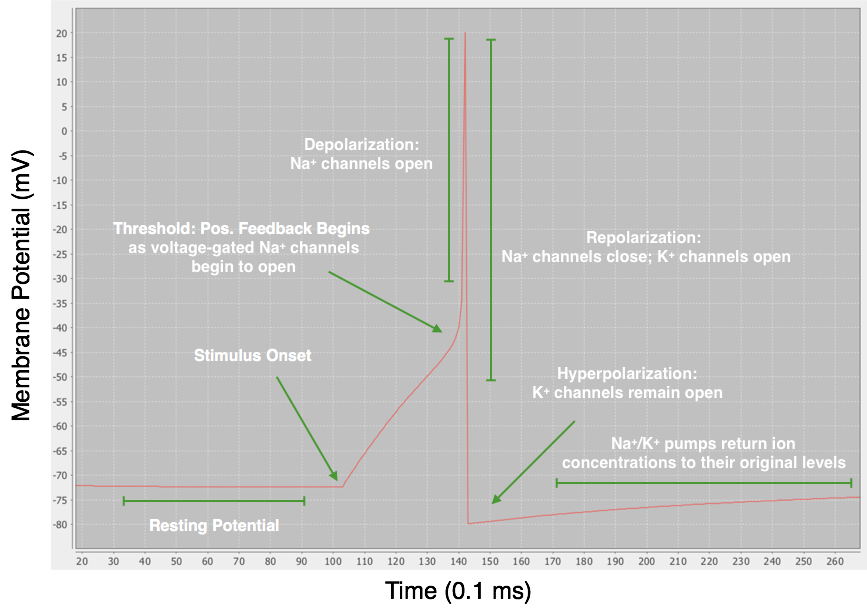
\includegraphics[width=\textwidth]{./images/ActionPotential.png}
	\caption[Simbrain screenshot]{A canonical action potential.}
	\label{ActPot}
\end{figure}


\section{Integrate and Fire Models}

The action potential is an all or nothing phenomena that almost always has the same amplitude. Furthermore the conditions for release of neurotransmitter are also always roughly the same. Thus if we are unconcerned with modeling the behavior of the membrane potential we can turn our attention entirely to this aspect of the neuron: Neurons integrate some input which then causes a response. If this response exceeds some threshold then an action potential is triggered resulting in post-synaptic events being fired along the neuron's outgoing synapses. That is why these are referred to as ``\textbf{Integrate and Fire (IF)}'' neurons. These models are focused exclusively on the all or nothing action potential. They are usually tuned to make spike timings and \textbf{inter-spike intervals (ISIs)} more precise and to match these signals to biology. These terms are \emph{not} concerned with matching the time-course of the membrane potential, or to ion channel behavior, or to known physiological values.\footnote{A notable exception might be the Izhikevich model, which was tuned so as to be able to replicate the membrane voltage traces of different kinds of neurons in addition to matching spike timing behavior.}

% Discuss this with Zoe before re-integrating. This is a key distinction, since those investigating spiking neural networks (SNNs) almost always choose some variety of integrate and fire. Why be interested in membrane potentials if the spike times are roughly the same when looking at a network-level phenomenon? Especially when models like the \textbf{adaptive exponential integrate and fire model} have been shown to very closely mimic the spike times of more sophisticated \textbf{Hodgkin-Huxley} models, which also model voltage traces and ion channel dynamics? One answer is this: many integrate and fire models do not explicitly simulate a neuron's \textbf{refractory period}, this is an explicit parameter of these models and typically they are not allowed to fire or receive inputs for some number of milliseconds (typically 1-3) after generating a spike.

\subsection{The Heaviside step function}

The spiking threshold model is the simplest of all spiking models. In fact it is so simple that it doesn't even meet many of the criteria listed in Fig. \ref{NeuComp}. It focuses on only one aspect of a spiking neuron, namely the all or nothing response that occurs in response to exceeding a threshold. There are no internal dynamics.

\begin{eqnarray*}
	r_j= \Theta\left(\sum_{i} r_i\,;\, \theta\right) \\
	\text{where: } \Theta\left( x\,;\, \theta \right) = \begin{cases}
	0 & x < \theta\\
	1 & x \geq \theta
	\end{cases}
\end{eqnarray*}

% Cohere with activation function chapter
Here $r$ is the activation value of the neuron, which takes on a discrete value of 1 or 0 based on the output of the Heaviside function ($\Theta(x)$) for the net input of the neuron (the sum of the outputs of neurons $i$ projecting onto $j$). Here we have parameterized the Heaviside function, which typically is 1 for values greater than or equal to 0 and 0 otherwise such that the argument passed to it (the net input in this case) must exceed a specified threshold for activation, $\theta$. Models using these neurons are the simplest of all spiking models and typically are not simulated continuously in time--instead being simulated by discrete iterations. This implies that networks composed of these neurons typically do not have dynamic synapses and instead in many ways closely resemble a typical ANN architecture. 

\subsection{Linear Integrate and Fire}

The linear integrate and fire model is one of the simplest of spiking neuron models that also has intrinsic dynamics. While we are not concerned here with fitting voltage traces for neurons, these models do attempt to capture precise spike timings, including timings that have interesting and varied behavior.

\begin{figure}[h]
\centering
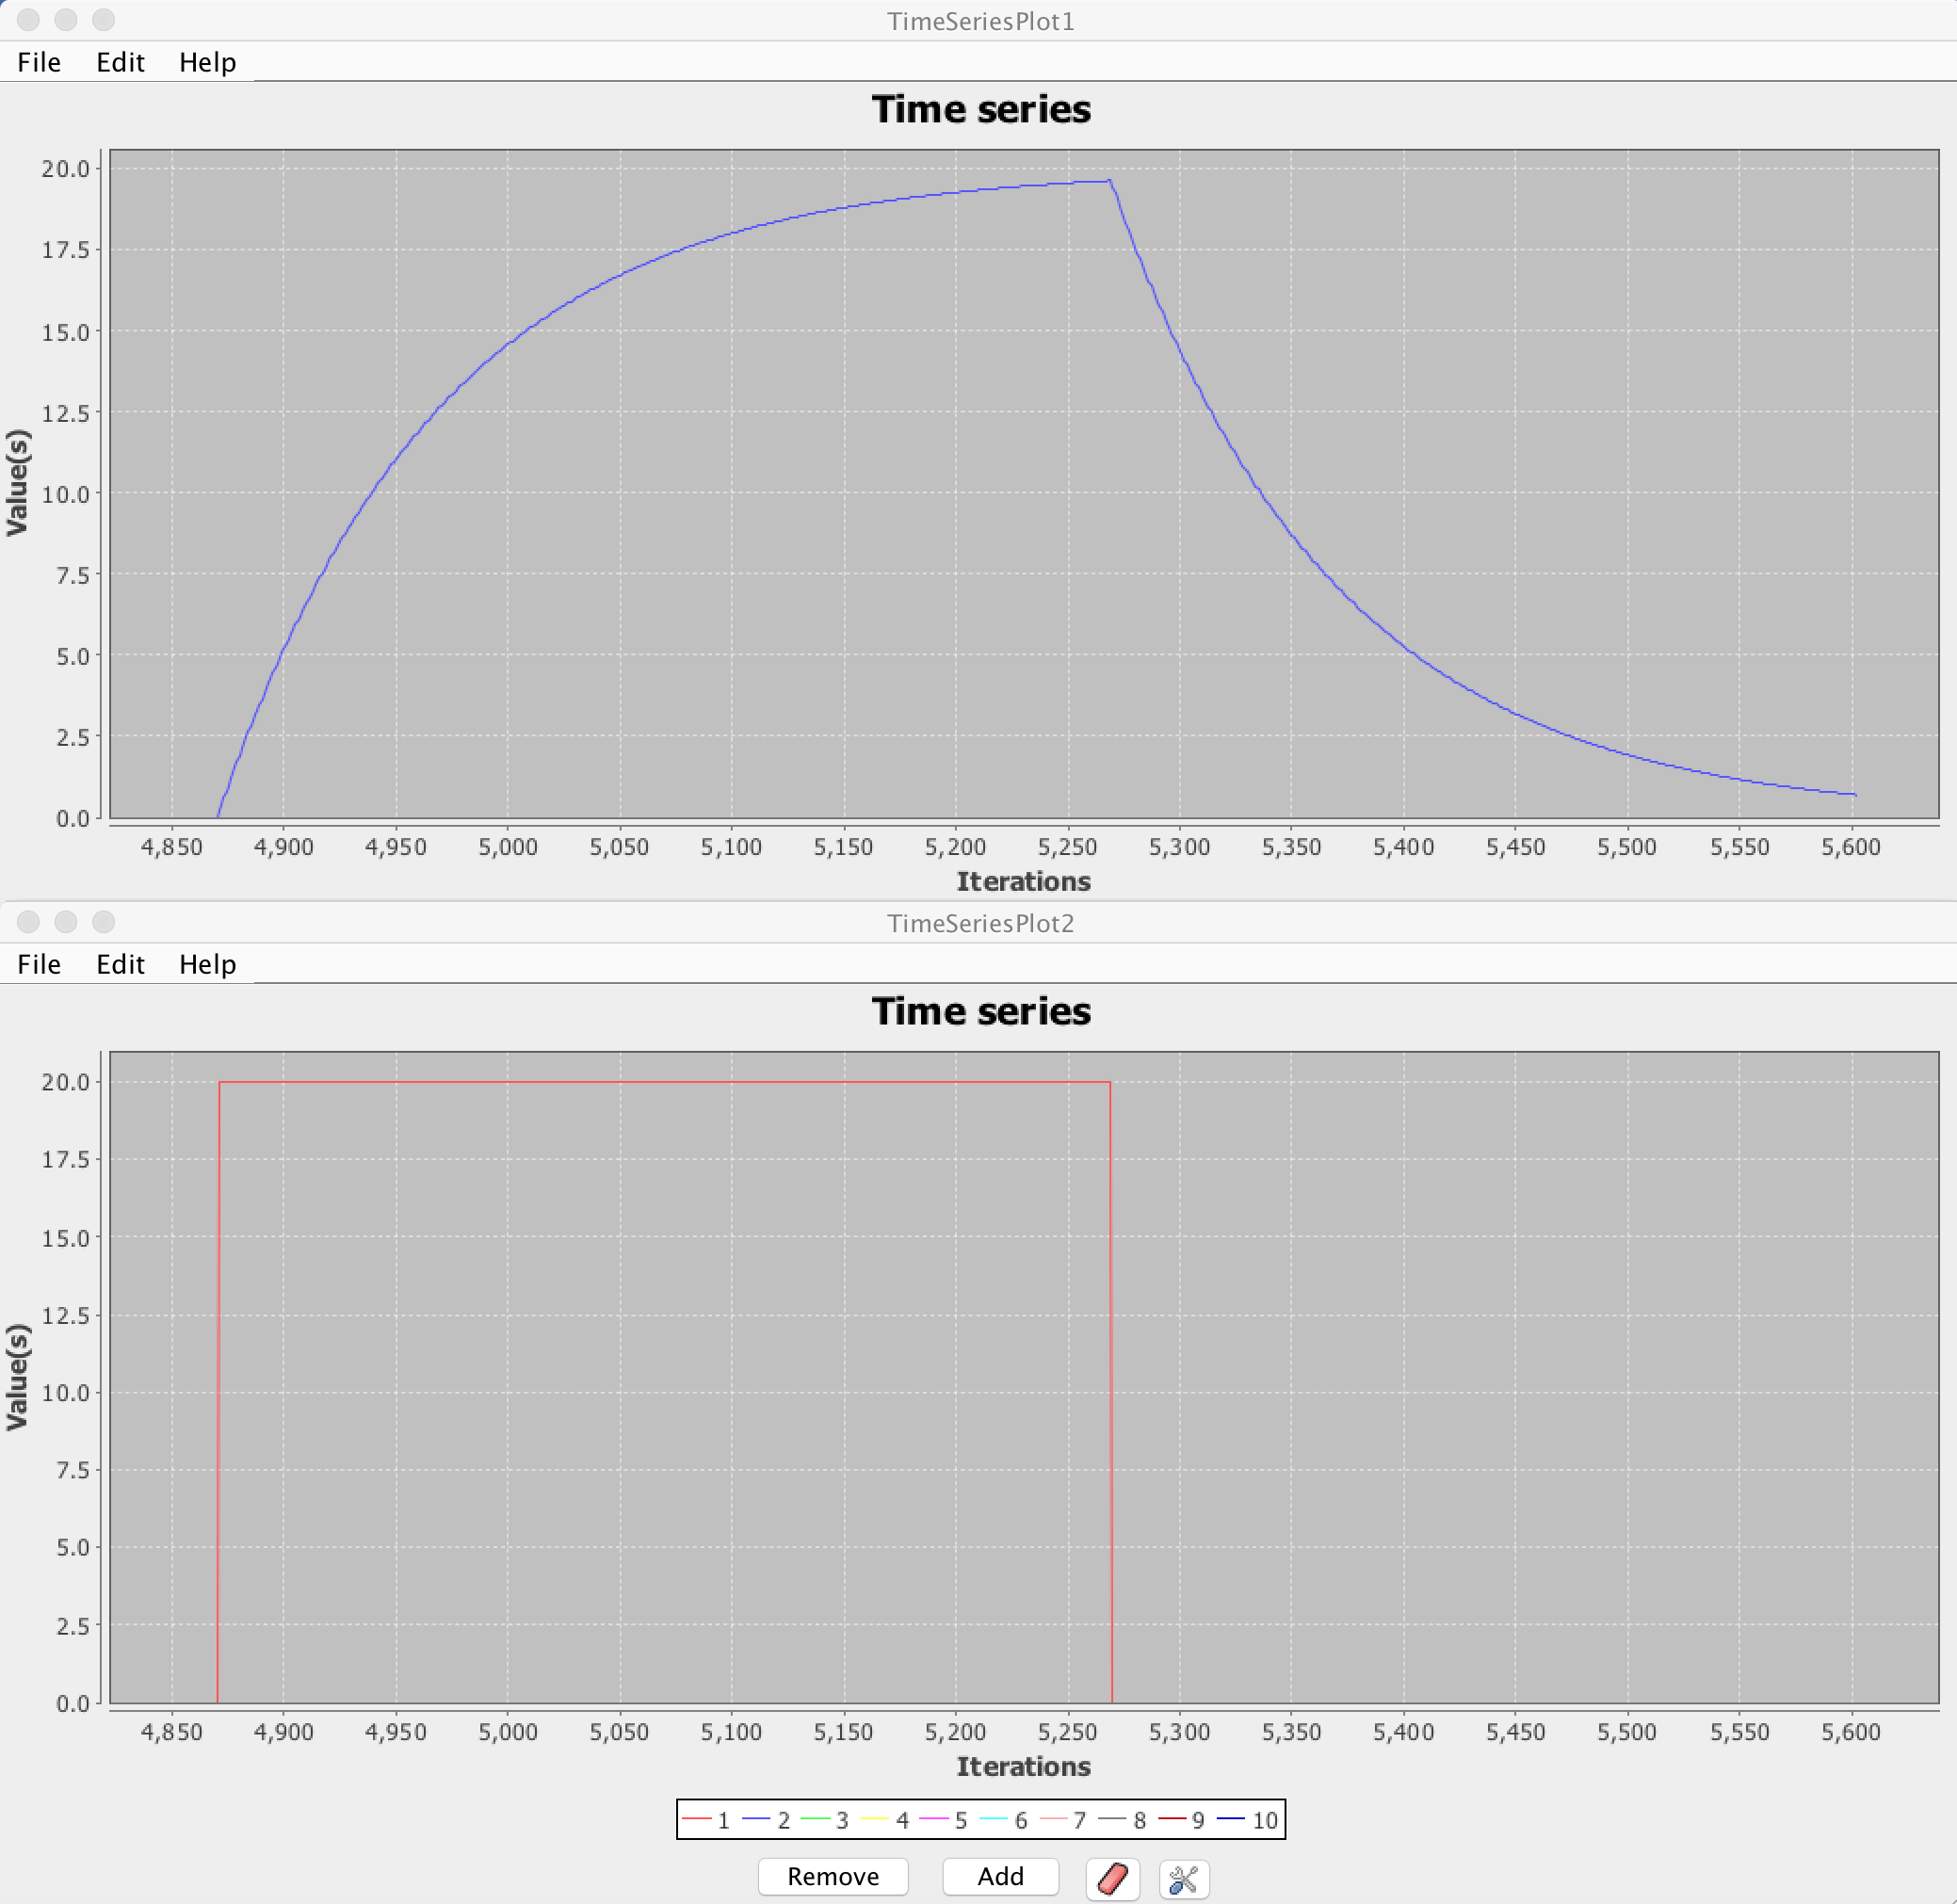
\includegraphics[width=\textwidth]{./images/LinIF_VoltTrace.png}
\caption[Simbrain screenshot by Zo\"e Tosi]{The response in the membrane potential of a linear integrate and fire neuron (blue/top) to a constant current injection (red/bottom). Notice the \emph{nonlinear} dynamical response in the LinIF neuron's membrane potential to a constant step in current. }
\label{LinIF_Traces}
\end{figure}

%\subsection{Quadratic Integrate and Fire}
%\subsubsection{Izhikevich}
%\subsection{Exponential Integrate and Fire}
%\subsubsection{The AdEx Model}

%\section{Complex Models: Hodgkin-Huxley and its Derivatives}
% the HH formalism
% \subsection{Hodgkin-Huxley}
%\subsection{Fitzhugh-Nagumo}
%\subsection{Morris-Lecar}

\section{Synapses with Spiking Neurons}

% Mention current vs. conductance based synapses.

\subsection{Spike Responses}

In the world of spiking neurons we are typically working in a continuous-time scenario rather than with discrete iterations. This presents a problem for the transfer of synaptic current from one neuron to another, since spikes are instantaneous events and as instantaneous events have an integral of $0$ for all finite values. Moreover, if we are in the business of simulating spiking neurons then we likely are concerned to some degree with the more realistic simulation of synapses as well, and in the real world synapses release neurotransmitters into the synaptic cleft over \emph{some duration}. Therefore for biological, mathematical, and practical reasons, a number of functions have been used to describe the post-synaptic response a synapse delivers to the post-synaptic neuron after a spike occurs.These are \textbf{spike response functions} or in Simbrain, ``spike responders''. 

Perhaps the most straightforward spike response function is an instantaneous jump and decay. Here it is assumed that upon the arrival of a spike a synapse instantly responds, proportional to its synaptic strength, and that response decays exponentially.

\begin{equation*}
\dot{q_{ij}} = -q_{ij} \tau_{psr} + w_{ij}\delta(t-t^n_i - \tau_{dly})
\end{equation*}

Or in closed form:
\begin{equation*}
q_{ij}(t) = \sum_{t^n_i < t} w_{ij}e^{-(t-t^n_i-\tau_{dly})/\tau_{psr}}
\end{equation*}

% Move up post-synaptic response and make sure it is clearly defined.
Here $q$ is the post-synaptic response: the value at each synapse, which the post-synaptic neuron $j$ sums over to determine the total current from synaptic responses. $\tau_{psr}$ is the time-constant of the exponential decay, $w_{ij}$ is the weight of the synapse connecting neurons $i$ and $j$. $t$ is current time while $t^n_i$ is the time of spike $n$ at neuron $i$ and $\tau_{dly}$ is the time-delay over the synapse. Lastly $\delta$ is the Dirac-delta function. This function is commonly used to represent spikes in continuous time systems, it is a function that is zero at all points on $[-\infty, \infty]$ except 0 where it is infinite. Thus its integral $\int_{-\infty}^{\infty} \delta(x)dx \;=\; 1$. This corresponds to a convolutional instantaneous jump and decay since the result of the application of this differential equation on the entire spike train of neuron $i$, $(n=1,...,N; t^n_i)$ is equivalent to the convolution of that spike train with an exponential kernel with a time constant of $\tau_{psr}$. This isn't always (nor does it have to be) treated as a convolution however and a maximum post synaptic response: $q_{max}$ can be established if so desired.

The instantaneous rise in post-synaptic response is not particularly realistic, since it takes some time for neurotrasmitter release to fully activate (not every synaptic vesicle is filled and touching the cell membrane ready for release after all). Thus there exist formalisms for modeling both the rise and the decay of a post-synaptic response. The simplest of these is the \emph{rise and decay} or \emph{alpha function}, which models both rise and decay using the same time constant. Having the same same time constant for both rise and decay is not particularly realistic, but it is also not an unreasonable approximation, and provides more realism than the instantaneous jump and decay function.

\begin{equation*}
\dot{q_{ij}} = -q_{ij}/\tau_{psr} + r \
\end{equation*}
\begin{equation*}
\dot{r} = -r/\tau_{psr} + w_{ij}\delta(t-t^n_i - \tau_{dly})
\end{equation*}

Or in closed form:
\begin{equation*}
q_{ij}(t) = \sum_{t^n_i < t} w_{ij}\left(\frac{t-t^n_i-\tau_{dly}}{\tau_{psr}}\right)e^{1-(t-t^n_i-\tau_{dly})/\tau_{psr}}
\end{equation*}

Here all variables are the same as in the previous section. Notice that we will reach our maximum response when the difference between the current time $t$ and the arrival of pre-synaptic spike $n$ from neuron $i$ ($t-t^n_i - \tau_{dly}$) is equal to our time constant $\tau_{psr}$. 

\begin{figure}[h]
\centering
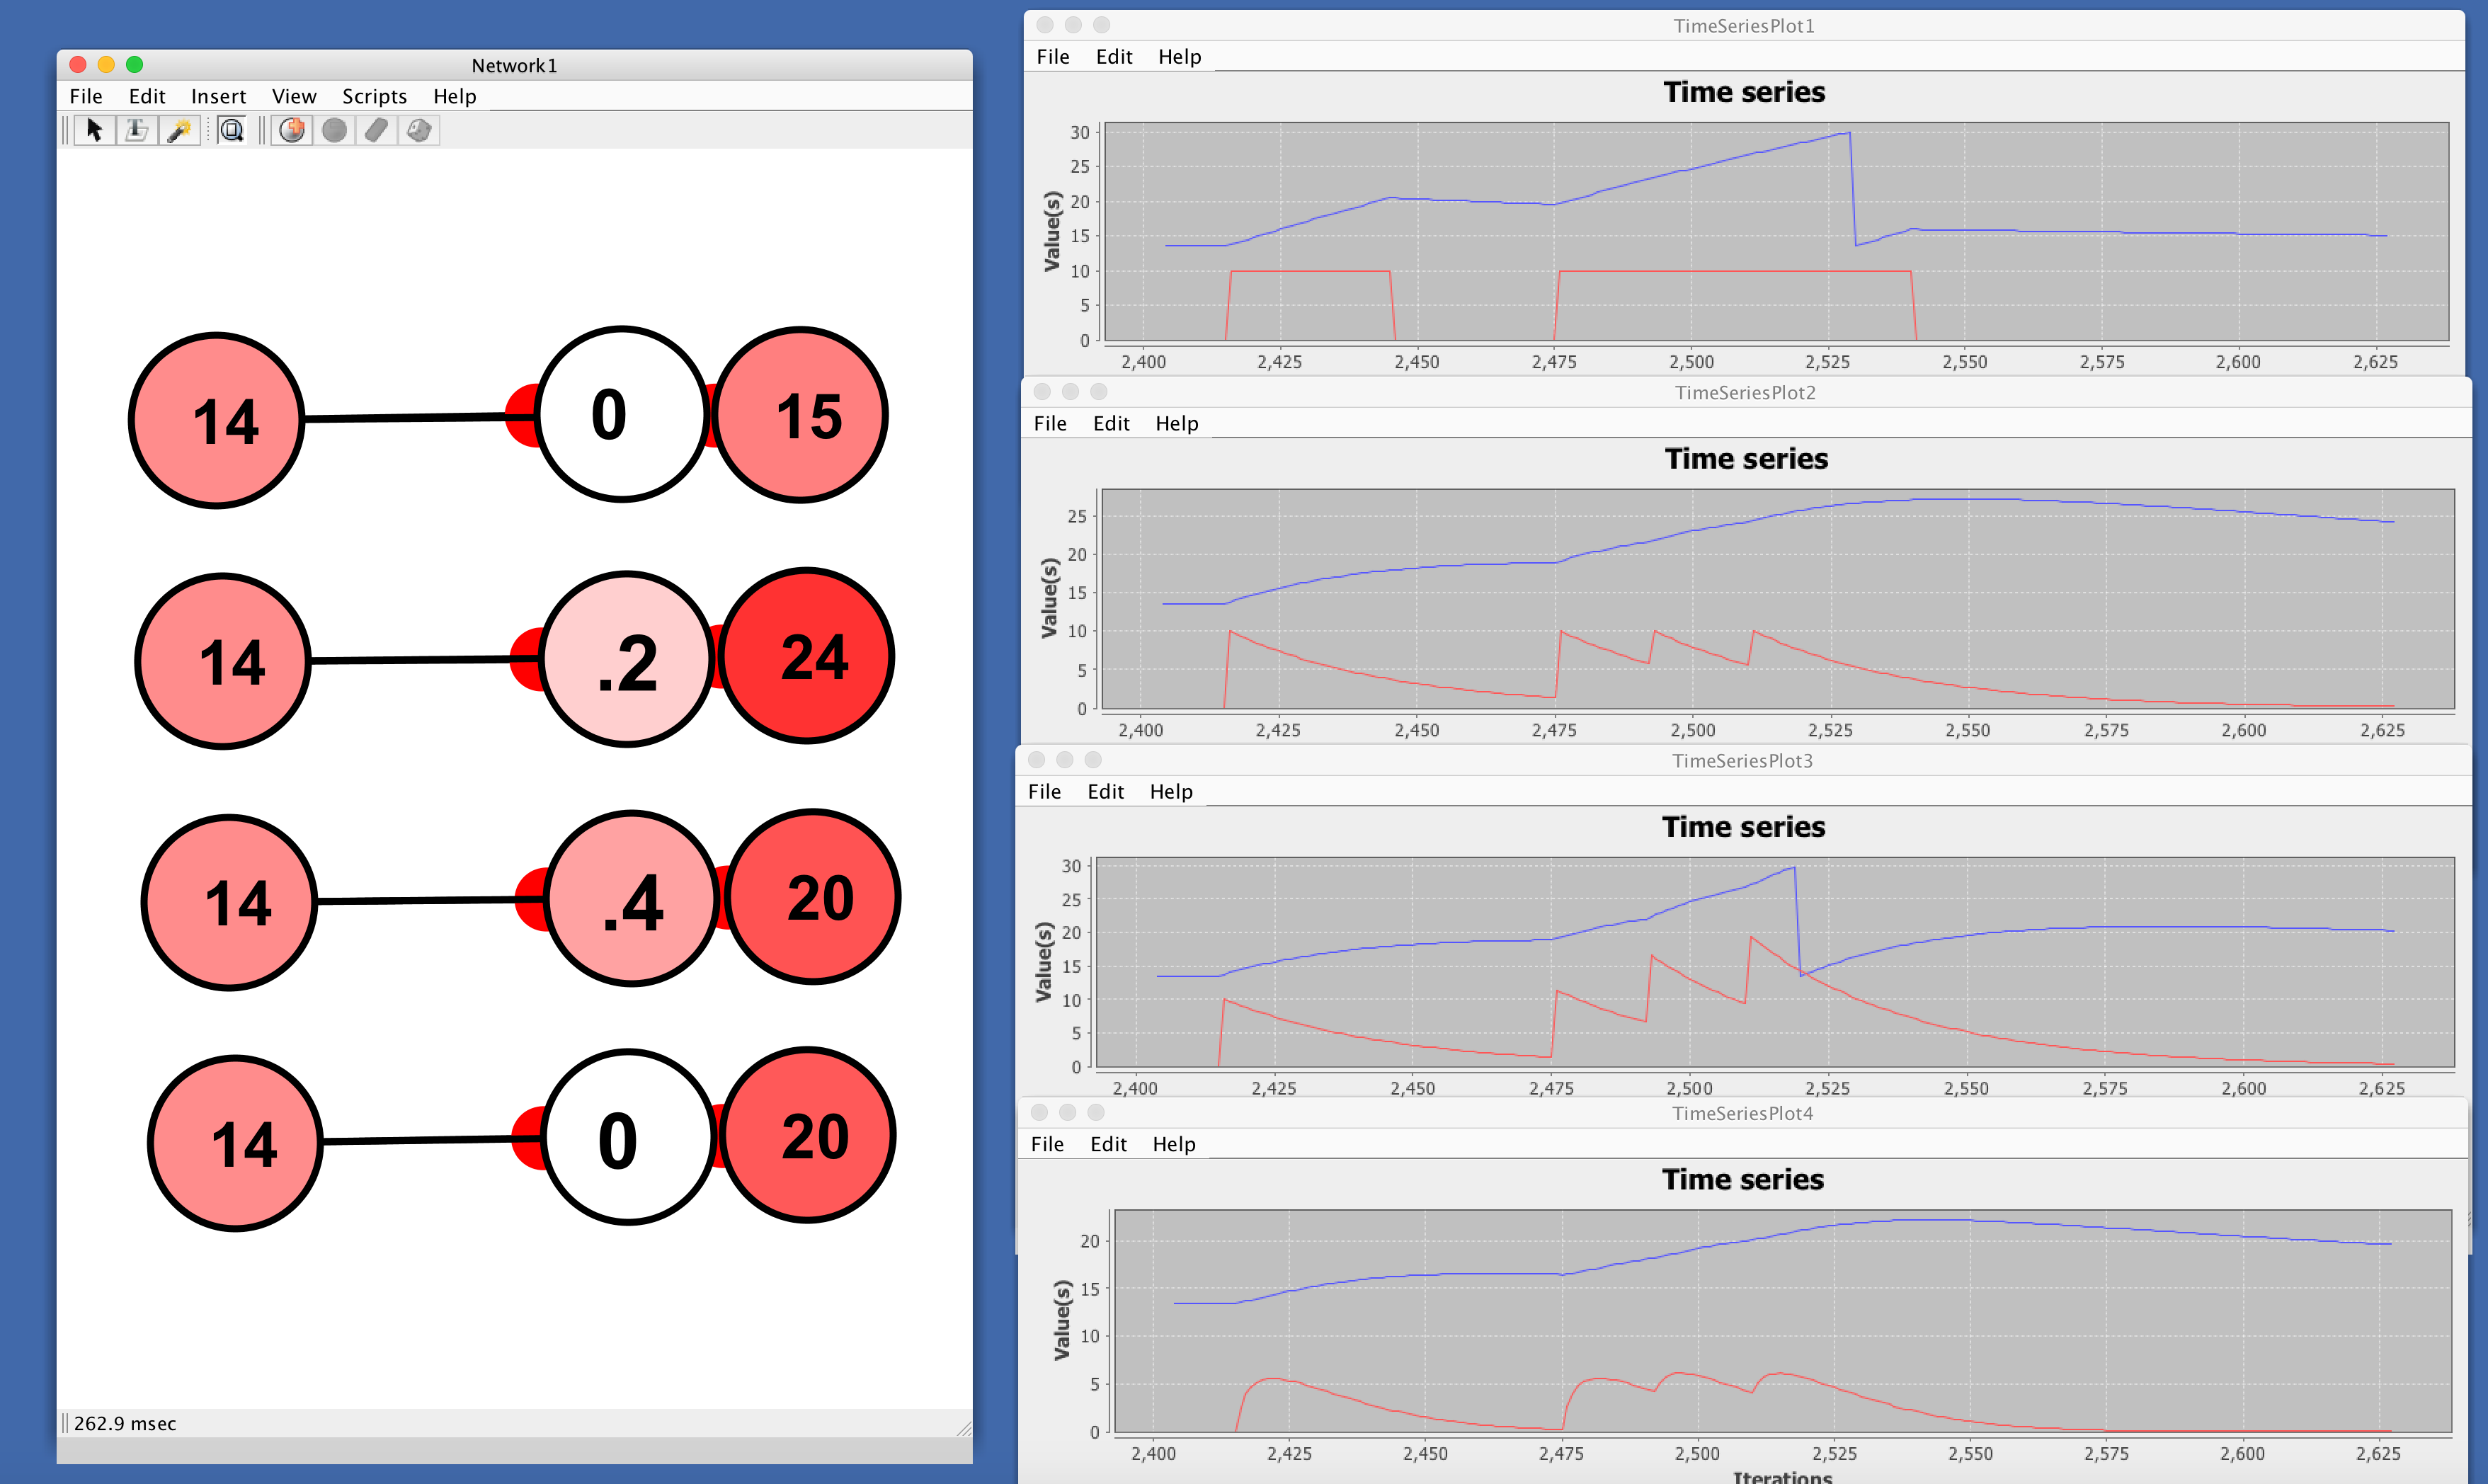
\includegraphics[width=\textwidth]{./images/SR_VoltTraces.png}
\caption[Simbrain screenshot by Zo\"e Tosi]{The post-synaptic responses for 4 different spike response mechanisms (red) plotted alongside the resulting change in post-synaptic membrane potential (blue). From top to bottom, we have a step-function, an instantaneous jump and decay with no convolution, a convolutional jump and decay, and a rise and decay function. Here post-synaptic neurons obeyed a linear integrate and fire rule. Notice the dynamical response from the post-synaptic IF neurons. }
\label{SR_Traces}
\end{figure}

%\subsection{Short-term plasticity}

\section{Long-term plasticity}

\subsection{Spike-Timing Dependent Plasticity (STDP)}

% Add extref to hebb
Spike-Timing Dependent Plasticity (STDP) is to spiking neurons what Hebbian learning is to continuous-valued nodes in a traditional artificial neural network. It is a mechanism for altering the strength of synaptic connections in a (typically) temporally asymmetric way such that certain pairings of spike times result in a change of the strength of a synapse. STDP or some variation thereof is believed to be a key component of a group of mechanisms underly memory, learning, and information processing in the brain. It is believed to play a key role in the development and maintenance of the specific synaptic structure of neural circuits.
% Add an intuitive discussion of STDP, the anti-causal stuff

% Could add a table and graphic here
 A Hebbian version of STDP is such that a spike in the pre-synaptic cell that temporally precedes a spike in the post-synaptic cell leads to a strengthening of the synapse while a spike in the post-synaptic cell which precedes a spike in the pre-synaptic cell leads to a weakening of the synapse. The former is known as \textbf{Long-Term Potentiation (LTP)} while the latter is referred to as \textbf{Long-Term Depression (LTD)}. This sort of relationship acts to create or reinforce positive temporal correlations between two neurons (at least in the case that the pre-synaptic cell is excitatory). However, STDP is not always Hebbian and can take on other forms. The  \textbf{STDP Window} is a function that takes as input the difference in spike times between a pre- and post-synaptic cell and outputs the change in the strength of the synapse connecting them. The familiar Hebbian window is the most common as it is ubiquitous among connections between two excitatory cells (which make up ~80\% of any given neuronal population in cortex). More exotic windows (of which there are many) are typically found at synapses where one or both of the cells involved are inhibitory. %(see \ref{sec:iSTDP} for a more detailed account).
 
\begin{figure} [h]
\centering
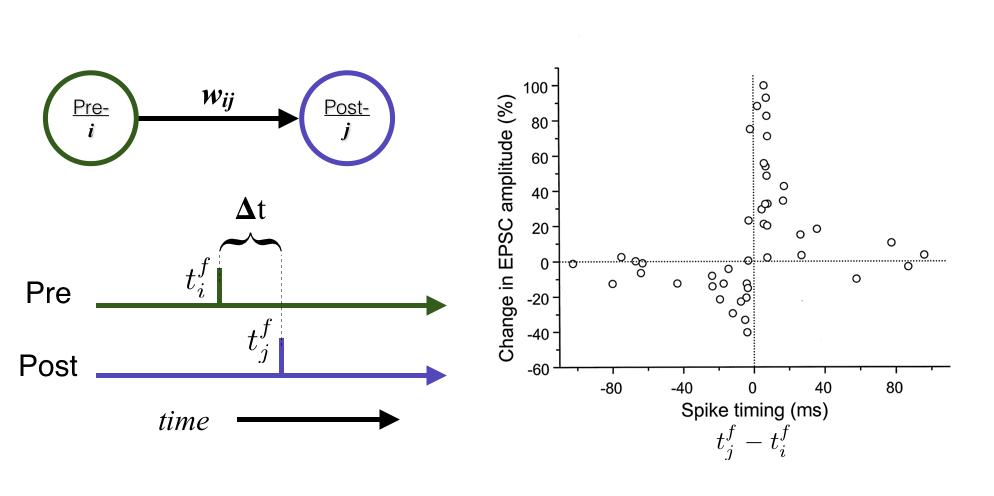
\includegraphics[width=\textwidth]{./images/STDP_intro_fig.png}
\caption[From Bi and Poo, 1998 \cite{bi1998synaptic}]{A diagram of STDP paired with empirical data showing the change in amplitude of the excitatory post-synaptic current (EPSC) produced by a synapse impinging on a neuron after repeated external stimulation of a pre- and post-synaptic neuron so as to force spikes in the two neurons with specific temporal differences. For each pair the stimulation protocol was repeated 60 times at a rate of 1 Hz and changes in synaptic efficacy were measured at 20 minutes after the protocol  \cite{bi1998synaptic}. A distinct shape can be seen whereby synapses where the pre-synaptic neuron was forced to spike immediately before its post-synaptic partner  experienced the greatest increase in strength with this increase dropping off exponentially with an increase in temporal difference between the pairs. Likewise pairs ordered such that the post-synaptic neuron fired first experienced a decrease in efficacy, which was most extreme if paired closely and also fell of exponentially with distance.}
\label{STDP_intro}
\end{figure}
\subsection{STDP}

In its most simple forms \glossary{STDP} is performed additively giving rise to the name ``Addititve STDP'' (or ``Add-STDP). Here we introduce the fundamental formalisms of STDP, which will appear in other variants and use add-STDP (sometimes referred to as ``vanilla'' STDP) as the particular instantiation.

Add-STDP refers to a broad set of models for STDP for which the change in the strength of a synapse is independent of the strength of that synapse. That is, weight changes occur in an \emph{additive} fashion. Add-STDP takes on the following form:

\begin{equation*}
\Delta w_{ij}  = \eta A_{+/-} exp(-|u| \tau_{+/-})
\end{equation*}
where $u = t^f_j-t^f_i$ and $t^f$ is the most recent time that either neuron $i$ or $j$ produced an action potential and $\eta$ is a learning rate. The $A_{+/-}$ term is one of two different constants depending upon the sign of $u$ (the difference in spike times between the pre- and post-synaptic cell). As the nomenclature implies this gives us $A_-$, which is typically negative reflecting LTD for negative $u$ (pre- fired after post-) and $A_+$ (typically positive reflecting LTP) for positive $u$ (post- fired after pre-). Similarly $\tau$ is a time-constant determining how quickly the effects of LTP and LTD decay over time in relation to the amount of time between pre- and post-synaptic spikes and as with $A$, $\tau_+$ and $\tau_-$ correspond to LTP or LTD. Together, this creates a piecewise exponential function centered (usually) on zero. This discrete formulation is applied instantaneously whenever neurons $i$ or $j$ fire. 

%\subsection{STDP Implementations/Variants}

%\subsubsection{Mlt-STDP}

%\subsubsection{Nlta-STDP}

%\subsubsection{Log-STDP}

%\subsection{Bienenstock, Cooper, and Monroe (BCM) Learning}

%\subsection{STDP with Inhibitory Neurons (iSTDP)} \label{sec:iSTDP}

%\begin{thebibliography}{}
%	
%	\bibitem{ } Bi, G. Q., \& Poo, M. M. (1998). Synaptic modifications in cultured hippocampal neurons: dependence on spike timing, synaptic strength, and postsynaptic cell type. {\it The Journal of neuroscience}, 18(24), 10464-10472.
%	\bibitem{} O'Reilly, RC, Munakata, Y, Frank, MJ, and Hazy TE. Computational Cognitive Neuroscience https://grey.colorado.edu/CompCogNeuro/index.php/CCNBook/Neuron
%	
%\end{thebibliography}


